\chapter{关系}
\begin{Def}
    设$A$与$B$为两个集合。一个从$A\times B$到$\{T,F\}$的映射$R$,称为从$A$到$B$的一个{\bfseries 二元关系}。
    $\forall (a,b) \in A \times B$,如果$(a,b)$在$R$下的象为$T$,则称$a$与$b$符合关系$R$,记为$aRb$;
    如果(a,b)在$R$下的象为$F$,则称$a$与$b$不符合关系$R$,记为$aR\!\!\! / b$。如
    果$A=B$,则称$R$为$A$上的二元关系。
  \end{Def}
  \begin{Example}
  设集合$X=\{1,2\}$,则$2^X$上的二元关系$\subseteq$可以定义为一个从$2^X\times
  2^X$到$\{T,F\}$的映射,

  $\subseteq(\{\phi\},\{\phi\})=T,\subseteq(\{\phi\},\{1\})=T,\subseteq(\{\phi\},\{2\})=T,\subseteq(\{\phi\},\{1,2\})=T,$

    $\subseteq(\{1\},\{\phi\})=F,\subseteq(\{1\},\{1\})=T,\subseteq(\{1\},\{2\})=F,\subseteq(\{1\},\{1,2\})=T,$

      $\subseteq(\{2\},\{\phi\})=F,\subseteq(\{2\},\{1\})=F,\subseteq(\{2\},\{2\})=T,\subseteq(\{2\},\{1,2\})=T,$

        $\subseteq(\{1,2\},\{\phi\})=F,\subseteq(\{1,2\},\{1\})=F,\subseteq(\{1,2\},\{2\})=F,\subseteq(\{1,2\},\{1,2\})=T$
      \end{Example}

  \begin{Def}
    设$A$与$B$为两个集合。$A\times B$的任一子集$R$称为从$A$到$B$的一个{\bfseries 二元关系}。如果$(a,b)\in R$,则称$a$与$b$符合关系$R$,记为$aRb$;如果$(a,b) \notin R$,则称$a$与$b$不符合关系$R$,并记为$aR\!\!\! / b$。
    如果$A=B$,则称$R$为$A$上的二元关系。
  \end{Def}
    \begin{Example}
  设集合$X=\{1,2\}$,则$2^X$上的二元关系$\subseteq$可以定义为$2^X\times
  2^X$的一个子集,

  \begin{equation*}
    \begin{split}
 \subseteq =& \{
 (\{\phi\},\{\phi\}),(\{\phi\},\{1\}),(\{\phi\},\{2\}),(\{\phi\},\{1,2\}),\\
 &(\{1\},\{1\}),(\{1\},\{1,2\}),(\{2\},\{2\}),(\{2\},\{1,2\}),\\
 &(\{1,2\},\{1,2\})
\}
    \end{split}
  \end{equation*}
\end{Example}

  \begin{Example}
    自然数集$\mathbb{N}$上的小于等于关系"$\leq$"为$\mathbb{N}$上的一个二元关系。
  \end{Example}
  \begin{Example}
    设$n$为任一给定的自然数。对任意的两个整数$m$,$k$,如果$m-k$能被$n$整除,则称$m$与$k$为模$n$同余,并记为$m\equiv k \pmod{n}$。
    显然,$m\equiv k \pmod{n}$当且仅当$m$被$n$除所得到的余数与$k$被$n$除所得到的余数相等。模$n$同余为$\mathbb{Z}$上的一个二元关系。
  \end{Example}

    \begin{Def}
    设$R \subseteq A \times B$,集合
    \[\{x \in A | \exists y \in B \text{使得} (x,y) \in R\}\]
    称为$R$的定义域,记为$dom(R)$; 集合
    \[\{y \in B | \exists x \in A \text{使得} (x,y) \in R\}\]
    称为$R$的值域,记为$ran(R)$。
  \end{Def}

    \begin{Def}
    设$A_1, A_2, \ldots, A_n$为$n$个集合,一个$A_1\times A_2 \times \cdots \times A_n$的子集$R$称为$A_1, A_2, \cdots, A_n$间的一个$n$元关系,每个$A_i$称为$R$的一个域。
  \end{Def}

  \begin{Def}
    集合$X$上的二元关系$R$称为自反的,如果对$X$的任意元素$x$都有$xRx$。
  \end{Def}
  \begin{Example}
    
    判断下列二元关系是否为自反的。设集合$X=\{1,2,3,4\}$,
  \begin{enumerate}
  \item 集合$X$上的二元关系$R=\{(1,2), (1,3), (1,4), (2,3),
    (2,4), (3,4)\}$ (不是)
  \item 集合$X$上的二元关系$R=\{(1,1), (1,2), (2,2),
    (2,4), (3,3), (4,4)\}$ (是)
  \item 集合$X$上的二元关系$R = \{(1,1), (2,3), (3,2)\}$ (不是)
  \item 集合$X$上的二元关系$R = \{(2,3)\}$ (不是)
  \item 集合$X$上的恒等关系$I_X = \{(1,1), (2,2), (3,3),(4,4)\}$ (是)
%  \item 设集合$X = \{0,1\}$, $2^X$上的二元关系$\subseteq$
  \end{enumerate}
  \end{Example}
  \begin{Def}
   集合$X$上的二元关系$R$称为反自反的,如果对$X$的任意元素$x$都有$(x,x) \notin R$。
 \end{Def}
 \begin{Example}   
    判断下列二元关系是否为反自反的。设集合$X=\{1,2,3,4\}$,
  \begin{enumerate}
  \item 集合$X$上的二元关系$R=\{(1,2), (1,3), (1,4), (2,3),
    (2,4), (3,4)\}$(是)
  \item 集合$X$上的二元关系$R=\{(1,1), (1,2), (2,2),
    (2,4), (3,3), (4,4)\}$ (不是)
  \item 集合$X$上的二元关系$R = \{(1,1), (2,3), (3,2)\}$(不是)
  \item 集合$X$上的二元关系$R = \{(2,3)\}$(是)
  \item 集合$X$上的恒等关系$I_X = \{(1,1), (2,2), (3,3),(4,4)\}$(不是)
%  \item 设集合$X = \{0,1\}$, $2^X$上的二元关系$\subseteq$
  \end{enumerate}
 \end{Example}

  \begin{Def}
    集合$X$上的二元关系$R$称为对称的,如果对$X$的任意元素$x$,$y$,只要$xRy$就有$yRx$。
  \end{Def}
  \begin{Example}
    判断下列二元关系是否为对称的。设集合$X=\{1,2,3,4\}$,
  \begin{enumerate}
  \item 集合$X$上的二元关系$R=\{(1,2), (1,3), (1,4), (2,3),
    (2,4), (3,4)\}$(不是)
  \item 集合$X$上的二元关系$R=\{(1,1), (1,2), (2,2),
    (2,4), (3,3), (4,4)\}$(不是)
  \item 集合$X$上的二元关系$R = \{(1,1), (2,3), (3,2)\}$(是)
  \item 集合$X$上的二元关系$R = \{(2,3)\}$(不是)
  \item 集合$X$上的恒等关系$I_X = \{(1,1), (2,2), (3,3),(4,4)\}$(是)
%  \item 设集合$X = \{0,1\}$, $2^X$上的二元关系$\subseteq$
  \end{enumerate}
\end{Example}
\begin{Def}
         集合$X$上的二元关系$R$称为反对称的,如果对$X$的任意元素$x$,$y$,$xRy$且$yRx$,则$x=y$。    
       \end{Def}
\begin{Example}
    判断下列二元关系是否为反对称的。设集合$X=\{1,2,3,4\}$,
  \begin{enumerate}
  \item 集合$X$上的二元关系$R=\{(1,2), (1,3), (1,4), (2,3),
    (2,4), (3,4)\}$(是)
  \item 集合$X$上的二元关系$R=\{(1,1), (1,2), (2,2),
    (2,4), (3,3), (4,4)\}$(是)
  \item 集合$X$上的二元关系$R = \{(1,1), (2,3), (3,2)\}$(不是)
  \item 集合$X$上的二元关系$R = \{(2,3)\}$(是)
  \item 集合$X$上的恒等关系$I_X = \{(1,1), (2,2), (3,3),(4,4)\}$(是)
%  \item 设集合$X = \{0,1\}$, $2^X$上的二元关系$\subseteq$
  \end{enumerate}
\end{Example}
\begin{Def}
        集合$X$上的二元关系$R$称为传递的,如果对$X$的任意元素$x$,$y$,$z$,只要$xRy$且$yRz$,就有$xRz$。
      \end{Def}
      \begin{Example}
    判断下列二元关系是否为传递的。设集合$X=\{1,2,3,4\}$,
  \begin{enumerate}
  \item 集合$X$上的二元关系$R=\{(1,2), (1,3), (1,4), (2,3),
    (2,4), (3,4)\}$(是)
  \item 集合$X$上的二元关系$R=\{(1,1), (1,2), (2,2),
    (2,4), (3,3), (4,4)\}$(不是)
  \item 集合$X$上的二元关系$R = \{(1,1), (2,3), (3,2)\}$(不是)
  \item 集合$X$上的二元关系$R = \{(2,3)\}$(是)
  \item 集合$X$上的恒等关系$I_X = \{(1,1), (2,2), (3,3),(4,4)\}$(是)
%  \item 设集合$X = \{0,1\}$, $2^X$上的二元关系$\subseteq$
  \end{enumerate}
\end{Example}
\begin{Def}
    设$R$为从集合$A$到集合$B$的二元关系,$R$的逆$R^{-1}$定义为从集合$B$到集合$A$的二元关系
    \[R^{-1}=\{(y,x)|(x,y)\in R\}\]
  \end{Def}
  \begin{Thm}
    设$R$为集合$X$上的二元关系,则$R$为对称的当且仅当$R=R^{-1}$。
  \end{Thm}  

    \begin{Def}
    设$R$为从集合$A$到集合$B$,$S$为从集合$B$到集合$C$的二元关系。$R$与$S$的合成
    $R\circ S$定义为从集合$A$到集合$C$的一个二元关系
    \[R\circ S = \{(x,z)\in A \times C |  \exists y \in B \text{使得} xRy \text{且} ySz\}\]
  \end{Def}
    \begin{Thm}
    设$R_1$,$R_2$,$R_3$分别为从集合$A$到集合$B$,从集合$B$到集合$C$,从集合$C$到集合$D$的二元关系,则
    \[(R_1 \circ R_2)\circ R_3 = R_1 \circ (R_2 \circ R_3)\]
  \end{Thm}
  \begin{Thm}
    设$R$为集合$X$上的一个二元关系,则$R$为传递的当且仅当$R\circ R \subseteq R$。
  \end{Thm}

   \begin{Def}
    设$X=\{x_1, x_2, \ldots, x_m\}$为一个包含$m$个元素的集合,$Y=\{y_1, y_2,
    \cdots, y_n\}$为一个包含$n$个元素的集合。令$R$为从$X$到$Y$的一个二元关系。
    由$R$定义一个$m \times n$矩阵$B = (b_{ij})$如下: $\forall (x_i, y_j) \in X \times Y$,
\[
    b_{ij}=
      \begin{cases}
        1,&\text{如果}x_iRy_j\\
        0,&\text{如果}x_iR\!\!\! / y_j
      \end{cases}
\]
    则矩阵$B$称为关系$R$的矩阵。
  \end{Def}

  \begin{Example}
    设集合$X=\{1,2,3,4\}$,$Y=\{a, b, c, d, e\}$, 从$X$到$Y$的关系\[S=\{(1,a),  (2, b), (2, d), (2, e), (3, a), (3, b), (3, d),  (3, e), (4,c), (4,d)\}\],则$S$的关系矩阵为?
  \end{Example}
  
  \begin{Example}
    设集合$X = \{1,2,3,4\}$,$R = \{(1,1),(1,2),(1,3),(1,4),(2,2),(2,4),(3,3),(4,2),(4,4)\}$,则$R$的关系矩阵为?
  \end{Example}

  \begin{Thm}
  设$B$为集合$X$上二元关系$R$的矩阵,则
  \begin{enumerate}
  \item $R$为自反的,当且仅当$B$的对角线上的全部元素都为1;
  \item $R$为反自反的,当且仅当$B$的对角线上的全部元素都为0;
  \item $R$为对称的,当且仅当$B$为对称矩阵;
  \item $R$为反对称的,当且仅当$i \neq j$时$b_{ij}$与$b_{ji}$不同时为1;
  \item $R$为传递的,当且仅当如果$b_{ij}=1$且$b_{jk}=1$,则$b_{ik}=1$。
  \end{enumerate}
\end{Thm}

关系除了用矩阵表示外,还可以用图来表示。设$X$和$Y$为有穷集
合,$R$为从$X$到$Y$的二元关系。当用图表示$R$时,先把$X$与$Y$的元素在纸
上用点表示,并在其旁边标上这个元素的名字。然后把$R$的任一序对$(x,y)$用
从代表$x$的点画一条指向代表$y$的点的矢线表示。这样就得到了一个由点、线
组成的“有向图”,称为关系$R$的图。注意,如果$(x,x)\in R$,则在代表$x$的点画一条又指向此点的矢线,称为环。
  \begin{Thm}
  设$R$为集合$X$上的二元关系,则
  \begin{enumerate}
  \item $R$为自反的,当且仅当$R$的图的每个顶点均有一个环;
  \item $R$为反自反的,当且仅当$R$的图中没有环;
  \item $R$为对称的,当且仅当$R$的图中任意两个不同顶点间有矢线,则必有两条方向相反的矢线;
  \item $R$为反对称的,当且仅当$R$的图中任意两个不同顶点间有矢线,则不能有两条方向相反的矢线;
  \item $R$为传递的,当且仅当在$R$的图中如果从某顶点沿矢线经两条矢线可到另一顶点,则从该顶点到另一顶点有一条矢线。
  \end{enumerate}
\end{Thm}

  \begin{Thm}
    设$B$为集合$X$上二元关系$R$的矩阵,则$R^{-1}$的矩阵为$B^{T}$。
  \end{Thm}


   \begin{Def}
    设$B$,$C$是两个布尔矩阵,$B$与$C$的逻辑乘为$B$与$C$的对应元素进行逻辑乘,所得到的布尔矩阵记为$B \land C$,即
    \begin{equation*}
      B \land C = (b_{ij} \land c_{ij})
    \end{equation*}
    $B$与$C$的逻辑加为$B$与$C$的对应元素进行逻辑加,所得到的布尔矩阵记为$B \lor C$,即
    \begin{equation*}
      B \lor C = (b_{ij} \lor c_{ij})
    \end{equation*}
  \end{Def}
  \begin{Thm}
    设$R$,$S$为从集合$X$到集合$Y$的二元关系,其矩阵分别为$B_R$和$B_S$。 $R\cup S$ 与$R \cap S$的矩阵分别为$B_{R\cup S}$,$B_{R\cap S}$,则
    \begin{equation*}
      B_{R\cup S}=B_R \lor B_S, B_{R\cap S}=B_R \land B_S
    \end{equation*}
  \end{Thm}
  \begin{Def}
    设$A$为$m\times p$布尔矩阵,$B$为$p \times n$布尔矩阵,$A$与$B$的布尔乘积$A \circ B$定义为矩阵$C$,其元素计算如下
    \begin{align*}
      c_{ij} &= (a_{i1}\land b_{1j}) \lor (a_{i2} \land b_{2j}) \lor \cdots \lor (a_{ip} \land b_{pj}), \\
      i &= 1,2,\cdots, m, j = 1,2,\cdots, n
    \end{align*}
  \end{Def}
  \begin{Thm}
    设$X, Y, Z$为有穷集合, $|X| =m$,$|Y|=p$,$|Z| = n$。$R$为从$X$到$Y$的二元
    关系, $S$为从$Y$到$Z$的二元关系,$R$,$S$,$R \circ S$的矩阵分别为$B_{R}$,$B_{S}$,$B_{R\circ S}$,则$B_{R\circ S} = B_R \circ B_S$。
  \end{Thm}
  \begin{Def}
    设$R$为集合$X$上的一个二元关系。$X$上的一切包含$R$的传递关系的交称为$R$的传递闭包,用$R^+$表示。即
    \begin{equation*}
      R^+ = \bigcap_{R \subseteq R' \text{且} R'\text{是传递的}}R'
    \end{equation*}
  \end{Def}
  \begin{Thm}
    设$R$为集合X上的一个二元关系,则关系$R$的传递闭包$R^+$为包含$R$的传递关系。
  \end{Thm}

  设$R$为集合$X$上的一个二元关系,$R$的非负整数次幂递归的定义如下:
  \[R^0=I_X,R^1=R,R^{n+1}=R^{n}\circ R\]

    \begin{Thm}
    设$R$为集合$X$上的一个二元关系,$a \in X$,$b \in X$,$n \geq 2$,则$(a,b) \in R^n$当且仅当存在$x_1\in X$,$x_2\in X$,$\ldots$,$x_{n-1}\in X$,使得$(a, x_1) \in R$,$(x_1, x_2)\in R$,  $\ldots$, $(x_{n-1}, b)\in R$。
  \end{Thm}
  \begin{proof}[证明]
  用数学归纳法证明,施归纳于$n$:

  当$n=2$时,由关系合成运算的定义知$(a,b)\in R^2$当且仅当存在$x_1\in X$使得$(a,x_1)\in R$且$(x_1, b)\in R$,结论成立。

   假设当$n=k$时定理的结论成立,往证当$n=k+1$时定理的结论也成立。
   由关系合成运算的定义知$(a,b)\in R^{k+1}$当且仅当存在$x\in X$使得$(a,x)\in R^k$且$(x, b)\in R$。 由归纳假设,$(a,x)\in R^k$当且仅当存在$x_1\in X$,$x_2\in X$,$\ldots$,$x_{k-1}\in X$,使得$(a, x_1) \in R$,$(x_1, x_2)\in R$,  $\ldots$, $(x_{k-1}, x)\in R$。 记$x_{k}=x$,则$(a,b)\in R^{k+1}$当且仅当存在$x_1\in X$,$x_2\in X$,$\ldots$,$x_{k-1}\in X$,$x_{k}\in X$,使得$(a, x_1) \in R,(x_1, x_2)\in R,\ldots,(x_{k-1}, x_k)\in R,(x_k, b)\in R$。
\end{proof}
  \begin{Thm}
    设$R$为集合$X$上的一个二元关系,则
    \begin{equation*}
      R^+ = \bigcup_{n=1}^\infty R^n = R \cup R^2 \cup R^3 \cup \cdots 
    \end{equation*}
  \end{Thm}
  \begin{Thm}
    设$R$为集合$X$上的一个二元关系,$|X| = n$,则\[R^+ = \bigcup_{i=1}^nR^i = R \cup R^2  \cup \cdots \cup R^n \]。
  \end{Thm}
  \begin{proof}[证明]
      只须证明对任一自然数$k > n$,有$R^k \subseteq \bigcup_{i=1}^nR^i$。
      为此,设$(a,b) \in R^k$,则存在$b_1, b_2, \cdots, b_{k-1} \in
      X$使得$(a,b_1) \in R$, $(b_1, b_2) \in R, \cdots, (b_{k-2}, b_{k-1})\in R,
      (b_{k-1}, b) \in R$。记$b_0 = a, b_k = b$。  $b_1,b_2, \cdots,
      b_{k-1}, b$是$X$中的$k$个元素,而$X$中仅有$n$个元素,$n < k$,所以$b_1,
      b_2, \cdots, b_{k-1}, b$中必有两个相等的元素。设$b_i=b_j$,$1 \leq i < j
      \leq k$。  于是,我们有$(a,b_1)\in R, \cdots, (b_{i-1}, b_i)\in R,
      (b_j, b_{j+1})\in R, \cdots, (b_{k-1},b)\in R$,故$(a,b)\in
      R^{k-(j-i)}$,$p_1=k-(j-i) < k$。  若$p_1 = k - (j - i) > n$, 则重复
      上述过程又有$p_2 < p_1$使得$(a,b) \in R^{p_2}$。  如此进行下去,必
      有$m \leq n$使得$(a,b) \in R^m$。所以,$R^k \subseteq
      \bigcup_{i=1}^nR^i$。  因此,$R^+=\bigcup_{i=1}^nR^i$。
  \end{proof}

    \begin{Thm}
    设$R$为集合$X$上的一个二元关系,$|X| = n$, $B$为$R$的关系矩阵,$B_{R^+}$为$R^+$的关系矩阵,简记为$B^+$,则
    \begin{equation*}
      B^+ = B \lor B^{(2)} \lor \cdots \lor B^{(n)}
    \end{equation*}
  \end{Thm}

  以下为计算集合$X$上关系$R$的传递闭包的算法。
   \begin{codebox}
    \Procname{$\proc{Transitive-Closure}(B)$}
    \zi \Comment $B$ is the zero-one $n \times n$ matrix for relation $R$
    \li $M \gets B$
    \li $A \gets M$
    \li \For $i \gets 2$ \To $n$
    \li \Do
        $M \gets M \circ B$
    \li $A \gets A \lor M$
    \End
    \li \Return A \Comment $A$ is the zero-one matrix for $R^+$
  \end{codebox}
  \begin{codebox}
    \Procname{$\proc{Warshall}(B)$}
    \zi \Comment $B$ is the zero-one $n \times n$ matrix for relation $R$
    \li $A \gets B$
    \li \For $k \gets 1$ \To $n$
    \li \Do
    \For $i \gets 1$ \To $n$
    \li \Do
    \For $j \gets 1$ \To $n$
    \li \Do
    $a_{ij} = a_{ij} \lor (a_{ik} \land a_{kj})$
    \End
    \End
    \End
    \li \Return A \Comment $A$ is the zero-one matrix for $R^+$
  \end{codebox}  

    \begin{codebox}
    \Procname{$\proc{Warshall}(B)$}
    \zi \Comment $B$ is the zero-one $n \times n$ matrix for relation $R$
    \li $A \gets B$
    \li \For $k \gets 1$ \To $n$
    \li \Do
    \For $i \gets 1$ \To $n$
    \li \Do
     \If $a_{ik} \isequal 1$
    \li \Then
    \For $j \gets 1$ \To $n$
    \li \Do
    $a_{ij} = a_{ij} \lor (a_{ik} \land a_{kj})$
    \End
    \End
    \End
    \End
    \li \Return A \Comment $A$ is the zero-one matrix for $R^+$
  \end{codebox}  
  \begin{Def}
    集合$X$上的二元关系$R$称为{\bfseries 等价关系},如果$R$同时满足以下三个性质:
    \begin{enumerate}
    \item $R$为自反的,即对$X$中的任意元素$x$,$xRx$;
    \item $R$为对称的,即对$X$中的任意元素$x$,$y$,如果$xRy$,则$yRx$;
    \item $R$为传递的,即对$X$中的任意元素$x$,$y$,$z$,如果$xRy$且$yRz$,则$xRz$。
    \end{enumerate}
  \end{Def}

  这是在我们这门课中迄今为止所学的所有概念中最重要的概念之一,是不是有点抽象?我们可以借助一个具体的例子,帮助我们理解这些抽象的概念。从小学到现在,我们是不是学了许多类似于“$\frac{1}{4}+\frac{1}{4}=\frac{1}{2}$”的等式?这里的等价关系就是从“$=$”抽象出来的。(1)$x=x$;(2)如果$x=y$,那么$y=x$;(3)如果$x=y$并且$y=z$,那么$x=z$。是不是显然成立呀?我们可以借助熟知的"="来理解等价关系的定义。
  \begin{Example}\label{mod}
    整数集$\mathbb{Z}$上的模$n$同余关系为$\mathbb{Z}$上的等价关系。
  \end{Example}
  \begin{proof}[证明]
    只需验证整数集$\mathbb{Z}$上的模$n$同余关系满足自反性,对称性和传递性。

    (1) 自反性成立,这是因为对任意的$m\in \mathbb{Z}$,$m\equiv m \pmod{n}$。(注:我们用$m\equiv k \pmod{n}$表示$m$与$k$模$n$同余,即$n | (m-k)$)

    (2) 对称性成立,这是因为对任意的$m\in \mathbb{Z}$,$k\in \mathbb{Z}$,如果$m\equiv k \pmod{n}$,则$n | (m-k)$,于是$n | (k-m)$,即$k\equiv m \pmod{n}$。

    (3) 传递性成立,这是因为对任意的$m\in \mathbb{Z}$,$k\in \mathbb{Z}$,$l\in \mathbb{Z}$,如果$m\equiv k \pmod{n}$并且$k\equiv l \pmod{n}$,则$n | (m-k)$并且$n | (k-l)$,从而$n | ((m-k) + (k-l))$,即$n | (m-l)$,因此$m\equiv l \pmod{n}$。
  \end{proof}
  \begin{Example}\label{number}
    设集合
    $X=\{1,2,3,4,5,6 \}$上的关系$R$定义如下:
    \begin{align*}
      R=&\{(1,1),(1,3),(1,5),(2,2),(2,4),(3,1),(3,3),(3,5),(4,2),\\
      &(4,4),(5,1),(5,3),(5,5),(6,6)\},
    \end{align*}
      则$R$为$X$上的等价关系。
    \end{Example}
    \begin{proof}[证法一]
      直接根据定义进行验证。
    \end{proof}
    \begin{proof}[证法二]
      画出$R$的关系图进行判断。

      
        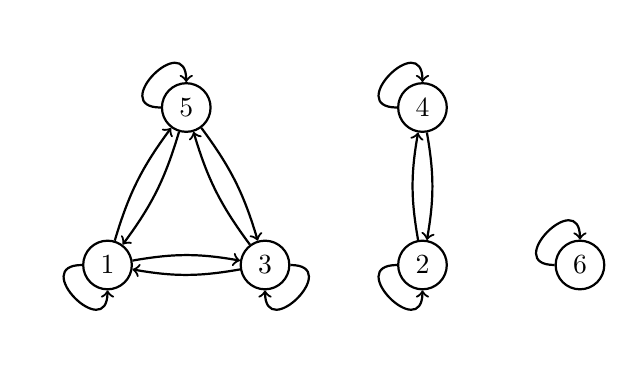
\begin{tikzpicture}[auto,
    specification/.style ={circle, draw, thick}]
   \node[specification] (A)  at (0,0)  {$1$};
   \node[specification] (B) at (2,0)  {$3$};
   \node[specification] (C)  at (1,2)  {$5$};
   \node[specification] (D)  at (4,0)  {$2$};
   \node[specification] (E)  at (4,2)  {$4$};
   \node[specification] (F)  at (6,0)  {$6$};
   
   \draw[thick, ->] (A) to [bend left = 10]  (B);
   \draw[thick, ->] (B) to [bend left = 10]  (A);

   \draw[thick, ->] (C) to [bend left = 10]  (B);
   \draw[thick, ->] (B) to [bend left = 10]  (C);
   
   
   \draw[thick, ->] (A) to [bend left = 10] (C);
   \draw[thick, ->] (C) to [bend left = 10] (A);
   
   \draw[thick, ->] (A) .. controls +(left:10mm) and +(down:10mm) ..  (A);
   \draw[thick, ->] (B) .. controls +(right:10mm) and +(down:10mm) ..  (B);
   \draw[thick, ->] (C) .. controls +(left:10mm) and  +(up:10mm) ..  (C);

   \draw[thick, ->] (D) to [bend left = 10] (E);
   \draw[thick, ->] (E) to [bend left = 10] (D);
   \draw[thick, ->] (D) .. controls +(left:10mm) and +(down:10mm) ..  (D);
   \draw[thick, ->] (E) .. controls +(left:10mm) and +(up:10mm) ..  (E);
   \draw[thick, ->] (F) .. controls +(left:10mm) and +(up:10mm) ..  (F);

\end{tikzpicture}

  
  (1)在$R$的图中,每个顶点均有一个环,这说明$R$为自反的;
  
  (2)在$R$的图中,如果任意两个不同顶点间有矢线,则必有两条方向相反的矢线,这说明$R$为对称的;

  (3)在$R$的图中,如果从某顶点沿矢线经两条矢线可到另一顶点,则从该顶点到另一顶点有一条矢线,这说明$R$为传递的。

    \end{proof}
    如果我们写个程序进行判断,首先要将该二元关系在计算机中表示出来。矩阵表示法为我们提供了一种解决方案。
    \begin{proof}[证法三]
      关系$R$的矩阵表示为
      \[B=\begin{bmatrix}
          1&0&1&0&1&0\\
          0&1&0&1&0&0\\
          1&0&1&0&1&0\\
          0&1&0&1&0&0\\
          1&0&1&0&1&0\\
          0&0&0&0&0&1
        \end{bmatrix}
      \]

      (1)$B$的对角线上的元素全为$1$说明$R$为自反的;

      (2)$B$为对称矩阵说明$R$为对称的;

      (3)

      \[B\circ B=\begin{bmatrix}
          1&0&1&0&1&0\\
          0&1&0&1&0&0\\
          1&0&1&0&1&0\\
          0&1&0&1&0&0\\
          1&0&1&0&1&0\\
          0&0&0&0&0&1
        \end{bmatrix}\circ\begin{bmatrix}
          1&0&1&0&1&0\\
          0&1&0&1&0&0\\
          1&0&1&0&1&0\\
          0&1&0&1&0&0\\
          1&0&1&0&1&0\\
          0&0&0&0&0&1
        \end{bmatrix}=\begin{bmatrix}
          1&0&1&0&1&0\\
          0&1&0&1&0&0\\
          1&0&1&0&1&0\\
          0&1&0&1&0&0\\
          1&0&1&0&1&0\\
          0&0&0&0&0&1
        \end{bmatrix}
      \]
      由$B\circ B$中的每个元素小于等于$B$中的每个元素知$R$为传递的。
    \end{proof}
  \begin{Def}
    设$\cong$为集合$X$上的一个等价关系,$x\in X$,$X$的子集
    \[E_x=\{y\in X | x \cong y\}\]称为$x$关于$\cong$的等价类,记为$[x]$,即
    \begin{equation*}
      [x] = \{y \in X | x \cong y\}
    \end{equation*}
  \end{Def}
  \begin{Example}
    在例\ref{mod}中我们已经知道模$4$同余关系为等价关系,试写出其所有等价类所构成的集合。
  \end{Example}
  \begin{proof}[解]
    模$4$同余关系所有等价类所构成的集合为$\{[0],[1],[2],[3]\}$,其中
    \begin{align*}
      [0]&=\{\cdots,-8,-4,0,4,8,\cdots\}\\
      [1]&=\{\cdots,-7,-3,1,5,9,\cdots\}\\
      [2]&=\{\cdots,-6,-2,2,6,10,\cdots\}\\
      [3]&=\{\cdots,-5,-1,3,7,11,\cdots\}
    \end{align*}
  \end{proof}
  \begin{Example}
    设集合
    $X=\{1,2,3,4,5,6 \}$上的关系$R$定义如下:
    \begin{align*}
      R=&\{(1,1),(1,3),(1,5),(2,2),(2,4),(3,1),(3,3),(3,5),(4,2),\\
      &(4,4),(5,1),(5,3),(5,5),(6,6)\},
    \end{align*}
      在例\ref{number}中,我们知道$R$为$X$上的等价关系,试写出其所有等价类所构成的集合。
    \end{Example}
    \begin{proof}[解]
      我们先尝试写出集合$X$上每个元素关于关系$R$的等价类:
      \begin{align*}
        [1]&=\{1,3,5\}\\
        [2]&=\{2,4\}\\
        [3]&=\{1,3,5\}\\
        [4]&=\{2,4\}\\
        [5]&=\{1,3,5\}\\
        [6]&=\{6\}
      \end{align*}
      你发现了什么?有重复!于是关系$R$的所有等价类所构成的集合为$\{[1],[2],[6]\}$, 即$\{\{1,3,5\},\{2,4\},\{6\}\}$。
    \end{proof}
    通过以上的例子,我们发现了以下的结论:
    \begin{Thm}
      设$\cong$为集合$X$上的一个等价关系,对任意的$x\in X$,$y\in X$,$x\cong y$当且仅当$[x]=[y]$。
    \end{Thm}
    \begin{proof}[证明]

      对任意的$x\in X$,$y\in X$,由$x\cong y$往证$[x]=[y]$。这里是要证明两个集合相等。对任意的$z\in [x]$,则$x\cong z$,由$\cong$的对称性知$z\cong x$,再由$\cong$的传递性及$x\cong y$知$z\cong y$,由$\cong$的对称性知$y\cong z$,从而$z\in [y]$。对任意的$z\in [y]$,则$y\cong z$,由$\cong$的传递性及$x\cong y$知$x\cong z$,从而$z\in [x]$。这证明了$[x]=[y]$。

      对任意的$x\in X$,$y\in X$,由$[x]=[y]$往证$x\cong y$。由$\cong$的自反性知$x\cong x$,从而$x\in [x]$,再由$[x]=[y]$知$x\in [y]$,从而$y\cong x$,由$\cong$的对称性得$x\cong y$。
    \end{proof}
   \begin{Def}
    设$X$为集合, $X$的一些非空子集形成的集族$\mathscr{A}$称为$X$的一个{\bfseries 划分},如果$\mathscr{A}$具有性质
    \begin{enumerate}
    \item $\forall A, B \in \mathscr{A}$,如果$A \neq B$,则$A \cap B = \phi$;
      \item $\bigcup_{A \in \mathscr{A}} = X$
    \end{enumerate}
  \end{Def}

  \begin{Example}
    集合
    \begin{equation*}
      \begin{split}
      \{&\{\cdots,-8,-4,0,4,8,\cdots\},\\
      &\{\cdots,-7,-3,1,5,9,\cdots\},\\
      &\{\cdots,-6,-2,2,6,10,\cdots\},\\
      &\{\cdots,-5,-1,3,7,11,\cdots\}\}
    \end{split}
  \end{equation*}
构成了整数集$\mathbb{Z}$的一个划分。
\end{Example}

  \begin{Example}
    集合$\{\{1,3,5\},\{2,4\},\{6\}\}$
构成了集合$X=\{1,2,3,4,5,6\}$的一个划分。
  \end{Example}

  \begin{Thm}\label{thm1}
    设$\cong$为集合$X$上的一个等价关系,则$\cong$的所有等价类的集合构成了集合$X$的一个划分。
  \end{Thm}
  \begin{proof}[证明]
    这就是要证明$\{[x]|x\in X\}$构成了集合$X$的一个划分。

    对任意$x\in X$,由$\cong$的自反性知$x\cong x$,从而$x\in [x]$,这证明了$[x]$非空。

    对任意的$x\in X$,$y\in X$,如果$[x]\neq [y]$,以下证明$[x]\cap [y]=\phi$。用反证法,假设$[x]\cap [y]\neq \phi$,则存在$z\in [x]\cap [y]$,于是$z\in [x]$并且$z\in [y]$。由$z\in [x]$知$x\cong z$,由$z\in [y]$知$y\cong z$。由$\cong$的对称性可得$z\cong y$,再由$\cong$的传递性可得$x\cong y$,从而$[x]=[y]$,矛盾。

    由对任意的$x\in X$,$x\in [x]$易知$\bigcup_{x\in X}[x]=X$。

    综上,我们证明了$\{[x]|x\in X\}$构成了集合$X$的一个划分。
  \end{proof}
  \begin{Thm}\label{thm2}
    设$\mathscr{A}$为集合$X$的一个划分,令\[\cong = \bigcup_{A\in \mathscr{A}}A\times A\]
    则$\cong$为集合$X$上的一个等价关系。
  \end{Thm}
  这个定理的符号不太好理解吧?在以后学习的过程中,遇到类似这个定理中的抽象的符号应该怎么办?具体的例子可以帮助我们很好的理解这些抽象的符号。例如,设集合$X=\{1,2,3,4,5,6\}$, $\mathscr{A}=\{\{1,3,5\},\{2,4\},\{6\}\}$为集合$X$的一个划分,则
  \begin{equation*}
    \begin{split}
      &\bigcup_{A\in \mathscr{A}}A\times A\\
      =&(\{1,3,5\} \times \{1,3,5\}) \cup (\{2,4\}\times \{2,4\}) \cup (\{6\}\times \{6\})\\
      =&\{(1,1),(1,3),(1,5),(3,1),(3,3),(3,5),(5,1),(5,3),(5,5),(2,2),(2,4),(4,2),(4,4),(6,6)\}
    \end{split}
  \end{equation*}
  为集合$X$上的一个等价关系。

  \begin{proof}[证明]
    这就是要验证$\cong$满足自反性、对称性和传递性。

    (1)对任意的$x\in X$,由$\mathscr{A}$为集合$X$的一个划分知存在$A\in \mathscr{A}$使得$x\in A$,从而$(x,x) \in A\times A$,于是, $(x,x)\in \bigcup_{A\in \mathscr{A}}A\times A$,这说明$\cong$满足自反性。

    (2)对任意的$x\in X$,$y\in X$,如果$(x,y)\in \bigcup_{A\in \mathscr{A}}A\times A$,那么存在$A\in \mathscr{A}$使得$(x,y)\in A\times A$,从而$(y,x)\in A\times A$,于是$(y,x)\in \bigcup_{A\in \mathscr{A}}A\times A$,这说明$\cong$满足对称性。

    (3)对任意的$x\in X$,$y\in X$,$z\in X$,如果$(x,y)\in \bigcup_{A\in \mathscr{A}}A\times A$,并且$(y,z)\in \bigcup_{A\in \mathscr{A}}A\times A$,那么存在$A\in \mathscr{A}$使得$(x,y)\in A\times A$,并且存在$B\in \mathscr{A}$使得$(y,z)\in B\times B$。于是,$x\in A$,$y\in A$,$y\in B$,$z\in B$。此时,必有$A=B$,否则$A\cap B=\phi$,这与$y\in A$并且$y\in B$矛盾。从而,$x\in A$,$z\in A$,因此,$(x,z)\in A\times A$,于是$(x,z)\in \bigcup_{A\in \mathscr{A}}A\times A$,这说明$\cong$满足传递性。
    
  \end{proof}

  本门课一个很重要的结论为“集合$X$上的所有等价关系之集与集合$X$的所有划分之集之间存在着一一对应的关系”。为了证明这个结论,我们需要构造一个从集合$X$上的所有二元关系之集到集合$X$的所有划分之集之间的一个双射。还记得我们学过的可逆映射的概念吗?一个映射为双射,当且仅当为该映射为可逆映射。于是我们可以构造一个从集合$X$上的所有二元关系之集到集合$X$的所有划分之集之间的一个可逆映射。还记得可逆映射的定义吗?

       设$f:X\to Y$为一个映射。如果存在一个映射$g:Y\to X$使得\[f\circ g = I_{Y} \text{且} g\circ f = I_{X},\]则称映射$f$为可逆的,而$g$称为$f$的逆映射。
借助于以上我们所学过的数学概念,我们有如下的定理:
 \begin{Thm}
    设$X$为一个集合,
    \begin{align*}
    \mathbb{R} &= \{\cong \subseteq X \times X | \cong\text{为集合}X\text{上的一个等价关系}\},\\
      \mathbb{A} &= \{\mathscr{A} \subseteq 2^X| \mathscr{A}\text{为集合}X\text{的一个划分}\},\\
      f &= \{(\cong, \{[x]_{\cong} | x \in X\})|\cong \in \mathbb{R}, [x]_{\cong}=\{y\in X | x \cong y\}\}\\
      g&=\{(\mathscr{A}, \bigcup_{A \in \mathscr{A}}A\times A)|\mathscr{A} \in \mathbb{A}\}
    \end{align*}
    则$f$为从$\mathbb{R}$到$\mathbb{A}$的双射,且$f^{-1}=g$。
  \end{Thm}
  如果我们能够完全理解该定理,并能够从“0”开始给出该定理的证明过程,即该定理所依赖的其他结论都可以给出证明,那么,整个前三章的内容,我们就有了一个很好的把握了。集中精力搞懂本课程的一些重要定理的证明过程,顺藤摸瓜,这些定理所依赖的其他结论也能够给出证明,直到可以从头开始说起,这对于提升我们的逻辑思维能力是很有帮助的。

  这是我们所遇到的第一个重要的定理。让我们先从理解这个定理开始吧。还记得我们应该怎样理解抽象的符号和术语吗?答案是尝试具体的例子。

  让我们尝试一个简单的集合:$X=\{1,2,3\}$。那么$\mathbb{R}$表示集合$X$上所有的等价关系构成的集合,这个集合是怎样的?这个问题不好回答吧?

  让我们先看$\mathbb{A}$吧。$\mathbb{A}$表示集合$X$的所有划分构成的集合。这个集合比较好写,你能写出答案吗?我的答案是这样的:

  \begin{equation*}
    \begin{split}
      \mathbb{A}=\{&\{\{1\},\{2\},\{3\}\},\\
      &\{\{1,2\},\{3\}\},\\
      &\{\{1,3\},\{2\}\},\\
      &\{\{2,3\},\{1\}\},\\
      &\{\{1,2,3\}\}\}
    \end{split}
  \end{equation*}

  对任意的$\mathscr{A}\in \mathbb{A}$,我们计算$\bigcup_{A \in \mathscr{A}}A\times A$,就可以得到$X$上的一个等价关系。该定理是在说,在$\mathbb{R}$和$\mathbb{A}$之间存在一个一一对应的关系,于是,我们有
  \begin{equation*}
    \begin{split}
      \mathbb{R}=\{&\{(1,1),(2,2),(3,3)\},\\
      &\{(1,1),(1,2),(2,1),(2,2),(3,3)\},\\
      &\{(1,1),(1,3),(3,1),(3,3),(2,2)\},\\
      &\{(2,2),(2,3),(3,2),(3,3),(1,1)\},\\
      &\{(1,1),(1,2),(1,3),(2,1),(2,2),(2,3),(3,1),(3,2),(3,3)\}\}      
    \end{split}
  \end{equation*}
  \begin{proof}[证明]
    \begin{enumerate}
    \item 证明$f$为映射。这就是要证明对于集合$X$上的任意一个等价关系$\cong$, 
      $\{[x]_{\cong}|x\in X\}$为集合$X$的一个划分。这就是定理\ref{thm1}。
    \item 证明$g$为映射。这就是要证明对于集合$X$的任意一个划分$\mathscr{A}$,
      $\bigcup_{A\in \mathscr{A}}A\times A$为集合$X$上的一个等价关系。这就是定理\ref{thm2}。
    \item 证明$g\circ f = I_{\mathbb{R}}$。这就是要证明对于集合$X$上的任意一个等
      价关系$\cong$,$\bigcup_{x\in X}[x]_{\cong}\times [x]_{\cong} = \cong$。

      这里是要证明两个集合相等。

      对任意的$x_1\in X$,$x_2\in X$,如果$(x_1,x_2)\in \bigcup_{x\in X}[x]_{\cong}\times [x]_{\cong}$,那么存在$x\in X$,$(x_1,x_2)\in [x]_{\cong}\times [x]_{\cong}$,于是$x_1\in [x]_{\cong}$并且$x_2\in [x]_{\cong}$,从而$x\cong x_1$并且$x\cong x_2$,由$\cong$的对称性知$x_1\cong x$,再由$\cong$的传递性知$x_1\cong x_2$,即$(x_1,x_2)\in \cong$。

      对任意的$x_1\in X$,$x_2\in X$,如果$(x_1,x_2)\in \cong$,则$x_1\cong x_2$,从而$x_2\in [x_1]_{\cong}$,由$\cong$的自反性知$x_1\cong x_1$,从而$x_1\in [x_1]_{\cong}$。于是,$(x_1,x_2)\in [x_1]_{\cong}\times [x_1]_{\cong}\subseteq \bigcup_{x\in X}[x]_{\cong}\times [x]_{\cong}$。
    \item 证明$f\circ g = I_{\mathbb{A}}$。这就是要证明对于集合$X$上的任意一个划分
      $\mathscr{A}$,关于等价关系$\bigcup_{A \in \mathscr{A}}A\times A$的等价类
      的集合就是$\mathscr{A}$。

      这里还是要证明两个集合相等。

      对任意的$x\in X$,设$[x]$为关于等价关系$\bigcup_{A \in \mathscr{A}}A\times A$的一个等价类,以下证明$[x]\in \mathscr{A}$。由$\bigcup_{A\in \mathscr{A}}A=X$知存在$A\in \mathscr{A}$使得$x\in A$。如果我们能够证明$[x]=A$,则$[x]\in \mathscr{A}$得证。对任意的$y\in [x]$,则$(x,y)\in \bigcup_{A \in \mathscr{A}}A\times A$。于是,存在$B\in \mathscr{A}$使得$(x,y)\in B\times B$,如果$B\neq A$,那么$x\in A$且$x\in B$,这与$A\cap B=\phi$矛盾,从而$B=A$,因此$y\in A$。反之,对任意的$y\in A$,则$(x,y)\in \bigcup_{A \in \mathscr{A}}A\times A$,从而$y\in [x]$。这证明了$[x]=A$,从而$[x]\in \mathscr{A}$。

      对任意的$A\in \mathscr{A}$,以下证明$A$为等价关系$\bigcup_{A \in \mathscr{A}}A\times A$的一个等价类。由$A$非空知,存在$x$,$x\in A$,以下证明$A=[x]$,这里$[x]$表示$x$关于等价关系$\bigcup_{A \in \mathscr{A}}A\times A$的一个等价类。对任意的$y\in A$,则$(x,y)\in A\times A \subseteq \bigcup_{A \in \mathscr{A}}A\times A$,从而$y\in [x]$。反之,如果$y\in [x]$,则由与前面相类似的,可以证明$y\in A$。这证明了$A=[x]$。
    \end{enumerate}
  \end{proof}
  \begin{Def}
    设$\cong$为$X$上的等价关系,$\cong$的所有等价类之集称为$X$对$\cong$的商集,记为$X/\cong$。即
    \[X/\cong = \{[x]|x\in X,[x]\text{为}x\text{关于}\cong \text{的等价类}\}\]
  \end{Def}

  \begin{Example}
    设集合$X=\{1,2,3,4,5,6\}$,$\cong$为集合$X$的等价关系,$X/\cong=\{\{1,2\},\{3,5\},\{4,6\}\}$,试求$\cong$。
  \end{Example}
  \begin{Def}
    集合$X$上的二元关系$R$称为{\bfseries 偏序关系},如果$R$同时满足以下三个性质:
    \begin{enumerate}
    \item $R$为自反的,即对$X$中的任意元素$x$,$xRx$;
    \item $R$为反对称的,即对$X$中的任意元素$x$,$y$,如果$xRy$且$yRx$,则$x=y$;
    \item $R$为传递的,即对$X$中的任意元素$x$,$y$,$z$,如果$xRy$且$yRz$,则$xRz$。
    \end{enumerate}
  \end{Def}
    \begin{Def}
    设$\leq$为集合$X$上的一个偏序关系,则称二元组$(X,\leq)$为一个{\bfseries 偏序集}。
  \end{Def}

    \begin{Example}
    实数集$\mathbb{R}$上通常的“小于等于”关系$\leq$为一个偏序关系,所以$(\mathbb{R},\leq)$为一个偏序集。
  \end{Example}
  \begin{Example}
    设$S$为一个集合,$S$的子集间的包含关系$\subseteq$为$2^S$上的一个偏序关系,所以$(2^{\mathbb{S}},\subseteq)$为一个偏序集。
  \end{Example}

  \begin{Example}
    设集合
    $X=\{a,b,c,d\}$上的关系$R$定义如下:
    \begin{equation*}
      R=\{(a,a),(a,b),(a,c),(a,d),(b,b),(b,d),(c,c),(c,d),(d,d)\}
    \end{equation*}
  \end{Example}
  则$R$为$X$上的偏序关系。

    \begin{Def}
    设$\leq$为集合$X$上的偏序关系,如果$\forall x, y \in X$,$x \leq y$与$y \leq x$至少有一个成立,则称$\leq$为$X$上的全序关系。相应的,二元组$(X,\leq)$称为全序集。
  \end{Def}

  \begin{Def}
    设$(X,\leq)$为一个偏序集,$A\subseteq X$。如果存在一个元素$s\in A$使得$\forall x \in A$有$x \leq s$,则称$s$为$A$的{\bfseries 最大元素};如果存在一个元素$t\in A$使得$\forall x \in A$有$t \leq x$,则称$t$为$A$的{\bfseries 最小元素}。
  \end{Def}

  我们用$x<y$表示$x\leq y$且$x\neq y$。
    \begin{Def}
    设$(X,\leq)$为一个偏序集,$A\subseteq X$。如果存在一个元素$s\in A$,在$A$中没
    有元素$x$使得$s < x$,则称$s$为$A$的{\bfseries 极大元素};如果存在一个元素$t\in A$,在$A$中没有元素$x$使得$x < t$,则称$t$为$A$的{\bfseries 极小元素}。
  \end{Def}

    \begin{Def}
    设$(X,\leq)$为一个偏序集,$A\subseteq X$。如果存在一个元素$s\in X$使得$\forall x \in A$有$x \leq s$,则称$s$为$A$的一个{\bfseries 上界};如果存在一个元素$t\in X$使得$\forall x \in A$有$t \leq x$,则称$t$为$A$的一个{\bfseries 下界}。
  \end{Def}
    \begin{Def}
      设$(X,\leq)$为一个偏序集,$A\subseteq X$。如果$A$有上界且$A$的一切上界之集有最小元素,则这个最小上界称为$A$的{\bfseries 上确界},记为$\sup A$;如果$A$有下界且$A$的一切下界之集有最大元素,则这个最大下界称为$A$的{\bfseries 下确界},记为$\inf A$。
  \end{Def}

  设$x, y, z \in \mathbb{R}$,则
   \begin{enumerate}
   \item   $x + y = y + x$
   \item   $(x + y) + z = x + (y + z)$
   \item   $0 + x = x + 0 = x$
   \item   $(-x) + x = x + (-x)= 0$
   \item   $x * y = y * x$
   \item   $(x * y) * z = x * (y *z)$
   \item   $1 * x = x * 1 = x$
   \item   $\forall x \in \mathbb{R} x \neq 0 \to x^{-1} * x = x * x^{-1} = 1$
   \item   $x* (y + z) = x * y + x * z$
   \item   $(y + z) * x = y * x + z * x$
   \item $x \leq x$
   \item $ x \leq y \land y \leq x \rightarrow x = y$
   \item $x \leq y \land y \leq z \rightarrow x \leq z$
   \item $x \leq y \lor y \leq x$ 
\item $x > y \rightarrow x + z > y + z$
\item $x > y \land z >0 \rightarrow x * z > y * z$
\item   $\forall A \subseteq \mathbb{R} (A \neq \phi \land \exists x \in \mathbb{R} (\forall y \in A (y \leq x)) \rightarrow \exists z \in R ((\forall y \in A (y \leq z) )\land ( \forall x \in \mathbb{R} (\forall y \in A (y \leq x) \rightarrow z \leq x))))$
\end{enumerate}

  \begin{Exercise}
设$R$为集合$X$上的一个二元关系,试证:$R$为一个等价关系当且仅当(1)对任意的$x\in X$,$xRx$;(2)对任意的$x\in X$,$y\in X$,$z\in X$,如果$xRy$且$xRz$,那么$yRz$。    
  \end{Exercise}

  \begin{Exercise}
  是否存在一个同时不满足自反性、对称性、反对称性、传递性和反自反性的二元关系?    
  \end{Exercise}
  \begin{Exercise}
  实数集上的“小于”关系$<$是否为反自反的?集合$X$的幂集$2^X$上的“真包含”
  关系$\subset$是否为反自反的?为什么?    
  \end{Exercise}

  \begin{Exercise}
  下列说法是否正确?若正确,请给出证明;若不正确,请说明理由。
  
  1)设$R$为集合$X$上的反自反的和传递的二元关系,则$R$为反对称的二元关系。
  
  2)设$R$为集合$X$上的对称的和传递的二元关系,则$R$为自反的二元关系。    
  \end{Exercise}

    \begin{Exercise}
  设集合$X = \{1,2,3\}$, $Y = \{1,2\}$,$S = \{f|f:X \to Y\}$。$S$上的二元关系$\cong$定义如下:$\forall f,g\in S$,$f \cong g$当且仅当\[I_m(f) = I_m(g)\]证明$\cong$为$S$上的等价关系,并求出等价类之集。    
  \end{Exercise}
  \begin{Exercise}
  设$X, Y, S$同习题3.4。$S$上的二元关系$\cong$定义如下:$\forall f,g\in S$,$f \cong g$当且仅当\[f(1) + f(2) + f(3) = g(1) + g(2) + g(3)\]证明$\cong$为$S$上的等价关系,并求出等价类之集。    
  \end{Exercise}
 \begin{Exercise}
  设$X, Y, S$同习题3.4。$S$上的二元关系$\cong$定义如下:$\forall f,g\in S$,$f \cong g$当且仅当\[\{f^{-1}(\{y\}) | y \in Y\} = \{g^{-1}(\{y\})|y \in Y\}\]证明$\cong$为$S$上的等价关系,并求出等价类之集。  
\end{Exercise}

  \begin{Exercise}
    是否存在一个偏序关系$\leq$,使$(X,\leq)$中有唯一极大元素,但没有最大元素?如
    果有,请给出一个具体例子;如果没有,请证明之。
  \end{Exercise}
  \begin{Exercise}
    令$X=\{a,b,c,d\}$,画出偏序集$(2^X,\subseteq)$的Hasse图。
  \end{Exercise}
 \begin{Exercise}
 令$S=\{1,2,\cdots,12\}$,画出偏序集$(S,|)$的Hasse图,其中$|$为整除关系。它有几
 个极大(小)元素?列出这些极大(小)元素。
  \end{Exercise}
  \begin{Exercise}
    偏序集$(X,\leq)$称为有序完备的,当且仅当$X$的每个有上界的非空子集有上确界。
    证明:偏序集$(X,\leq)$为有序完备的当且仅当对$X$的每个有下界的非空子集有下确
    界。
  \end{Exercise}

\setcounter{Exercise}{0}
  \begin{Exercise}
设$R$为集合$X$上的一个二元关系,试证:$R$为一个等价关系当且仅当(1)对任意的$x\in X$,$xRx$;(2)对任意的$x\in X$,$y\in X$,$z\in X$,如果$xRy$且$xRz$,那么$yRz$。    
  \end{Exercise}

\begin{proof}[证明]

  设$R$为等价关系,往证(1)(2)成立。由$R$为自反的知(1)成立。其次,对任意的$x\in X$,$y\in X$,$z\in X$,如果$xRy$且$xRz$,由$R$的对称性知$yRx$,再由$R$的传递性知$yRz$。

  假设(1)(2)成立,往证$R$为等价关系。由(1)知$R$为自反的。其次,对任意的$x\in X$,$y\in X$,如果$xRy$,由(1)知$xRx$,再由(2)知$yRx$,这说明$R$为对称的。最后,对任意的$x\in X$,$y\in X$,$z\in X$,如果$xRy$并且$yRz$,由$R$为对称的知$yRx$,再由(2)知$xRz$,这说明$R$为传递的。
  

  
\end{proof}

%%% Local Variables:
%%% mode: latex
%%% TeX-master: "book_chapter3"
%%% End:

\input{p113-theorem3-6-6-exercise}
\begin{proof}[证法一]
  根据传递闭包的定义进行证明。只需证$R\circ S$为包含$R\cup S$的所有传递关系的交。

  首先证明$R\circ S$为包含$R\cup S$的传递关系。对任意的$a\in X,c\in X$,如果$(a,c)\in R\cup S$,则$(a,c)\in R$或者$(a,c)\in S$。如果$(a,c)\in R$,此时由$S$为等价关系知$(c,c)\in S$,从而$(a,c)\in R\circ S$; 如果$(a,c)\in S$,此时由$R$为等价关系知$(a,a)\in R$,从而$(a,c)\in R\circ S$。这证明了$R\cup S\subseteq R\circ S$。由$R\circ S$为等价关系知$R\circ S$为传递的。

  其次,设$T$为任意一个包含$R\cup S$的传递关系,证明$R\circ S \subseteq T$。对任意的$a\in X,c\in X$,如果$(a,c)\in R\circ S$,则存在$b\in X$,$(a,b)\in R$并且$(b,c)\in S$。从而$(a,b)\in R\cup S \subseteq T$,$(b,c)\in R\cup S \subseteq T$,再由$T$为传递关系知$(a,b)\in T$。
\end{proof}

\begin{proof}[证法二]
  先证$R\circ S\subseteq (R\cup S)^+$。

  对任意的$a\in X,c\in X$,如果$(a,c)\in R\circ S$,则存在$b\in X$,$(a,b)\in R$并且$(b,c)\in S$,从而$(a,b)\in R\cup S$并且$(b,c)\in R\cup S$,于是$(a,c)\in (R\cup S)^2 \subseteq (R\cup S)^+$。

  再证$(R\cup S)^+\subseteq R\circ S$。

  对任意的$a\in X,c\in X$,由$(a,c)\in (R\cup S)^+$,往证$(a,c)\in R\circ S$。

  对任意的$a\in X,c\in X$,如果$(a,c)\in (R\cup S)^+$,则存在自然数$n$,$n\geq 1$, $(a,c)\in (R\cup S)^n$。

  以下用数学归纳法证明,对任意的自然数$n$,$n\geq 1$,$(R\cup S)^n\subseteq R\circ S$。

  (1)当$n=1$时,对任意的$a\in X,c\in X$,如果$(a,c)\in R\cup S$,则$(a,c)\in R$或者$(a,c)\in S$。如果$(a,c)\in R$,此时由$S$为等价关系知$(c,c)\in S$,从而$(a,c)\in R\circ S$; 如果$(a,c)\in S$,此时由$R$为等价关系知$(a,a)\in R$,从而$(a,c)\in R\circ S$。

  (2)假设当$n=k(k\geq 1)$时结论成立,往证当$n=k+1$时结论也成立。

  由$R$,$S$,$R\circ S$都为$X$上的等价关系知,$S\circ R=S^{-1}\circ R^{-1}=(R\circ S)^{-1}=R\circ S$。

  对任意的$a\in X,c\in X$,如果$(a,c)\in (R\cup S)^{k+1}=(R\cup S)^k\circ (R\cup S)$,则存在$b\in X$,$(a,b)\in (R\cup S)^k$并且$(b,c)\in (R\cup S)$。由归纳假设,$(a,b)\in R\circ S$。如果$(b,c)\in R$,那么$(a,c)\in (R\circ S)\circ R = R\circ (S\circ R) = R\circ (R\circ S) = (R\circ R)\circ S = R^2\circ S \subseteq R\circ S$;如果$(b,c)\in S$,那么$(a,c)\in (R\circ S)\circ S = R\circ (S\circ S) = R\circ S^2 \subseteq R\circ S$。
  

  
\end{proof}

%%% Local Variables:
%%% mode: latex
%%% TeX-master: "book_chapter3"
%%% End:
      \chapter{}

%%% Local Variables:
%%% mode: latex
%%% TeX-master: "book_chapter3"
%%% End:

